% !TeX spellcheck = en_US


\section{Benchmark: block size versus write speed}
\label{sec:blocksize}
The Wupper GUI makes it possible for the users to configure the block size value. This appendix shows how much effect the block size have on the write speed. 

During a DMA write action (FPGA$\,\to\,$PC), a transfer request is transferred from the host to the FPGA, therefore a write descriptor is setup. This descriptor contains information such as memory addresses, direction and the size of the payload, i.e. the amount of data to be transfered. The descriptor is then handled by Wupper, and the data transfer to host initiated. The size of the payload is in this case also the block size. For example when users choose to have a block size of 1 KB, the request gets completed after 1 KB of data had been transferred to host. Subsequently a new header will be created and repeated until the throughput measurement is stopped by the user. 
A plot of the block size versus write speed is shown below in Figure~\ref{fig:blocksizeplot}. One can clearly observe from this plot that the block size have effect on the write speed. This is somehow expected as there is an overhead due to the request of those blocks, hence the more data get transfer per request, the better the PCIe bandwidth is exploited. The bigger the block size is, the faster the write speed gets. The throughput obviously saturates at a level close to the theoretical maximum speed defined by an 8 lane PCIe Gen3 link (64 Gbps).

\begin{figure}[h]
	
	\centering
	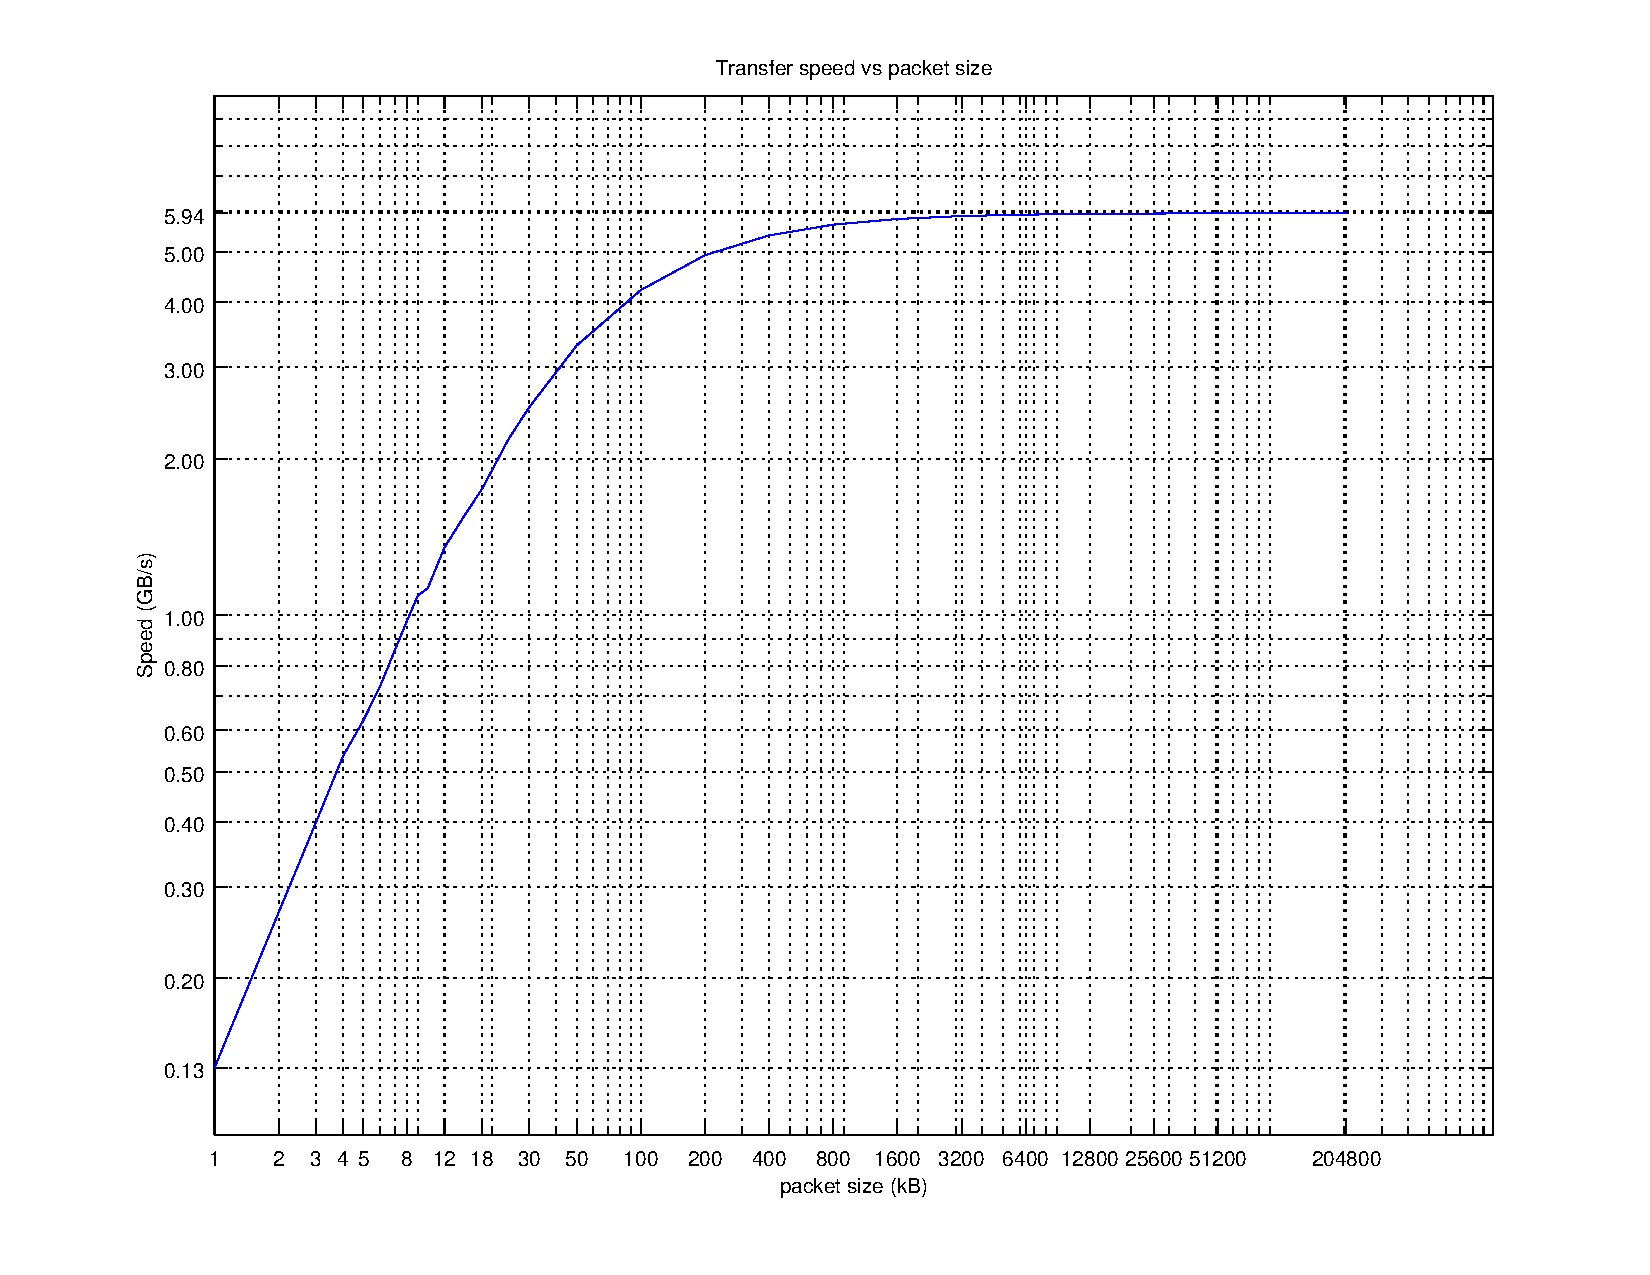
\includegraphics[width = 1 \textwidth]{figures/blocksize_plot.pdf}	
	\caption{upfifo and downfifo are full.}
	\label{fig:blocksizeplot}
\end{figure}


\newpage

\section{Problem solving: solution on different stream congestion and data corruption}

This appendix shows the approach of the problem during verification of the example application. During a write action (FPGA$\,\to\,$PC), data flows into the PC memory. But when a DMA read action (PC$\,\to\,$FPGA) is performed, the Wupper tool got stuck. The result of debugging the tool shows that the strange behaviour occurs during a $DMA\_WAIT$ function. This function waits on the assertion of the descriptor completion signal from the Wupper core, this signal informs the host PC that the DMA action is completed. The signal comes from the Wupper core, this allows to take a closer look at the HDL module.
The ILA core allows to fire an immediate trigger to capture the status of the signals. First thing that attract attention is that both FIFO's are full as shown below in Figure~\ref{fig:fifofull}.

\begin{figure}[h]
	
	\centering
	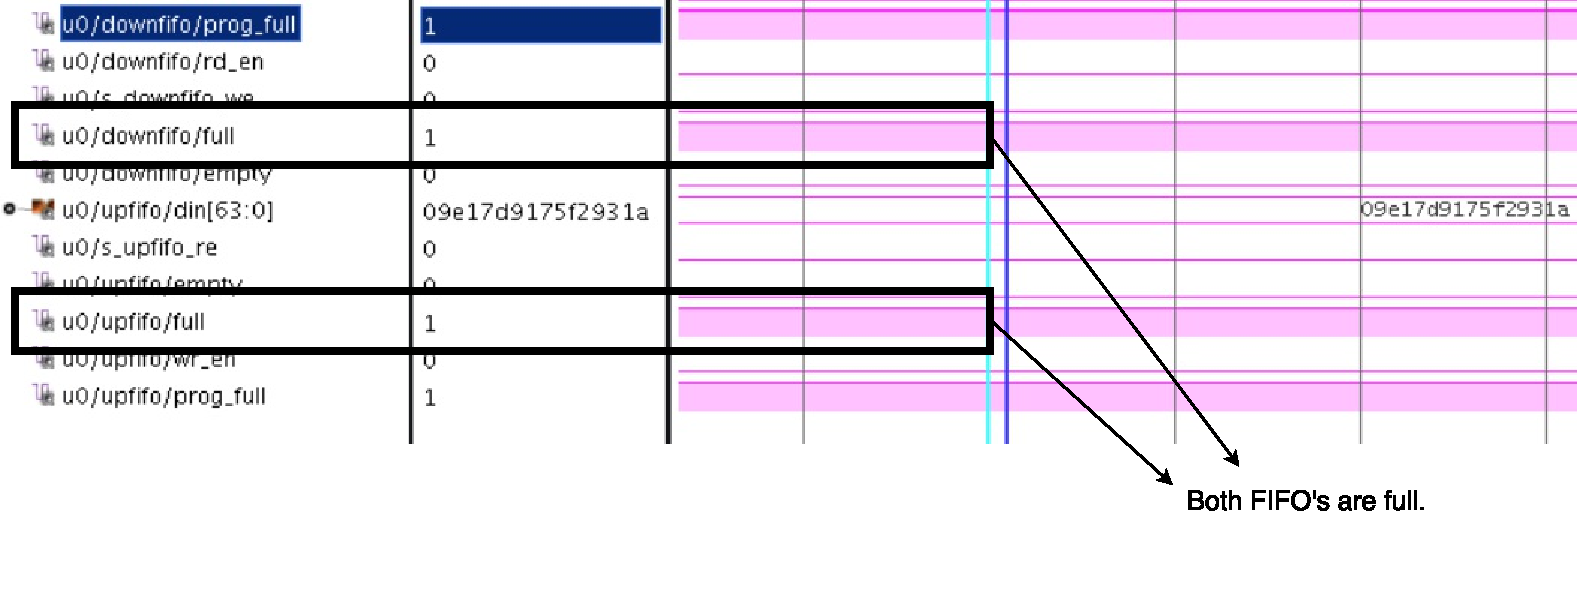
\includegraphics[width = 1 \textwidth]{figures/fifos_full.pdf}	
	\caption{upfifo and downfifo are full.}
	\label{fig:fifofull}
\end{figure}


 In order to resolve this issue, three changes where required:

\begin{itemize}
	\item Editing the $DMA\_WAIT$ function: the function contains a timer which stops executing itself after a certain period and returns an error message. This measure allows the user clarity. 
	
	\item Increasing the depth of the Up FIFO: by expanding the Up FIFO, the example application have more capacity so more room for processing data.
	
	\item Adding application enable block in the example application: As described before in paragraph 3.2.1, to prevent data congestion in the example application.

\end{itemize}
 


\newpage
%\subsection{Testing methodology}
%Pipelining problems
%Clock domain crossing
%DMA Backpressure
%Simulation
%Block size plot
%Real time testing(Chipscope)
%\subsection{Chipscope flow}
%How to setup debug nets
%Screenshot ILA
%How to trigger
\section{Application Base Address Region}
\label{sec:bar2}

The registers in BAR2, which is shown below in Table ~\ref{tab:dma_register_map_bar2}, is dedicated to user application.

\begin{longtabu} to \textwidth {|X[1.5,l]|X[7,l]|X[1,l]|X[1,l]|X[5,l]|}
	\hline
	\textbf{Address} & {\textbf{Name/Field}} &\textbf{Bits} &{\textbf{Type}} &\textbf{Description} \\
	\hline
	\endhead
	
	\multicolumn{5}{|c|}{Bar2} \\
	\hline
	
	
	
	0x0000 & REG\_BOARD\_ID &	39:0 & R & Board ID  \\
	\hline
	0x0010 & REG\_STATUS\_LEDS & 7:0 & R/W & Board GPIO Leds\\
	\hline
	0x0040 & REG\_CARD\_TYPE & 63:0 & R & Card type information\\
	\hline
	\multicolumn{5}{|c|}{Monitor Registers} \\
	\hline	
	0x0300 & REG\_PLL\_LOCK &
	19:0 & R & PLL lock status\\
	\hline
	0x1060 & INT\_TEST\_2 &
	any & T & Fire a test MSIx interrupt \#2 \\
	\hline
	0x1070 & INT\_TEST\_3 &
	any & T & Fire a test MSIx interrupt \#3 \\
	\hline
	\multicolumn{5}{|c|}{Example application register} \\
	\hline
	0x2000 & REG\_LFSR\_SEED\_0 &
	63:0 & R/W & Seed value 127:0\\
	\hline
	0x2010 & REG\_LFSR\_SEED\_1 &
	63:0 & R/W & Seed value 256:128\\
	\hline
	0x2020 & REG\_APP\_MUX  &
	1 & R/W & Select of the application multiplexer\\
	\hline
	0x2030 & REG\_LFSR\_LOAD\_SEED &
	1 & R/W & Initialize the seed value in to the data generator\\
	\hline
	0x2040 & REG\_APP\_ENABLE &
	2:0 & R/W & Enables the application\\
	\hline
	0x310 & REG\_CORE\_TEMPERATURE &
	4:0 & R & XADC temperature core\\
	
	
	\hline									
	\caption{Register map BAR2}\label{tab:dma_register_map_bar2} \\
\end{longtabu}

\newpage


